% =====================================================================
% Deep Double Descent - COMP34312 Poster Coursework
% A2 LANDSCAPE, beamerposter, customised UoM purple theme.
% Compile: pdflatex poster-landscape.tex
% =====================================================================
\documentclass[final]{beamer}

\usepackage[orientation=landscape,size=a2,scale=0.95]{beamerposter}
\usepackage{lmodern}
\usepackage[T1]{fontenc}
\usepackage[utf8]{inputenc}
\usepackage{amsmath,amssymb,amsthm,bm,mathtools}
\usepackage{xcolor}
\usepackage{graphicx}
\usepackage{tikz}
\usepackage{microtype}
\usepackage{booktabs}
\usepackage[english]{babel}
\usepackage{calc}
\usepackage{ragged2e}
\usetikzlibrary{shapes,arrows.meta,positioning,calc,backgrounds,fit,decorations.pathreplacing}

% ----- Colours: University of Manchester palette + supporting accents -----
\definecolor{uompurple}{HTML}{660099}     % Primary UoM purple
\definecolor{uompurpleDark}{HTML}{3F0066} % Deep variant for headers
\definecolor{uompurplePale}{HTML}{F2EAF7} % Background tint
\definecolor{uomgrey}{HTML}{2A2A33}       % Body text
\definecolor{uommuted}{HTML}{555A66}      % Captions/secondary
\definecolor{uomline}{HTML}{D9DCE5}       % Dividers
\definecolor{accentcoral}{HTML}{D1495B}   % Critical regime
\definecolor{accentteal}{HTML}{087E8B}    % Underparameterised
\definecolor{accentgreen}{HTML}{2E7D32}   % Overparameterised
\definecolor{accentgold}{HTML}{B98300}    % Caveats
\definecolor{accentblue}{HTML}{2D6CDF}    % Sample-wise

% ----- Theme overrides -----
\setbeamercolor{normal text}{fg=uomgrey,bg=white}
\setbeamercolor{block title}{fg=white,bg=uompurple}
\setbeamercolor{block body}{fg=uomgrey,bg=white}
\setbeamerfont{block title}{size=\large,series=\bfseries}
\setbeamerfont{block body}{size=\small}
\setbeamertemplate{itemize items}[circle]
\setbeamertemplate{itemize item}{\textcolor{uompurple}{\textbullet}}
\setbeamertemplate{itemize subitem}{\textcolor{uommuted}{\(\cdot\)}}
\setbeamertemplate{navigation symbols}{}

% Rounded block titles + body, with left-edge purple accent stripe under body
\setbeamertemplate{block begin}{
  \par\vskip0.4ex
  \begin{beamercolorbox}[rounded=true,leftskip=0.5cm,colsep*=0.5ex,wd=\linewidth]{block title}%
    \usebeamerfont*{block title}\insertblocktitle%
  \end{beamercolorbox}%
  \nointerlineskip\vskip-0.2ex%
  \usebeamerfont{block body}%
  \begin{beamercolorbox}[rounded=true,leftskip=0.35cm,rightskip=0.35cm,colsep*=0.5ex,sep=0.4ex,vmode]{block body}%
    \vbox{}\vskip-0.3ex%
}
\setbeamertemplate{block end}{%
  \end{beamercolorbox}\vskip0.3ex%
}

% Decorative section-number badge for block titles
\newcommand{\sectnum}[1]{\textcolor{accentgold}{\bfseries #1}\,}

% ----- Custom commands -----
\newcommand{\kw}[1]{\textcolor{uompurple}{\textbf{#1}}}
\newcommand{\eyebrow}[1]{{\color{uompurple}\scriptsize\bfseries\MakeUppercase{#1}}\par\vspace{-0.2ex}}
\newcommand{\takeaway}[1]{%
  \begin{center}\colorbox{uompurplePale}{\parbox{0.96\linewidth}{\centering\itshape\textcolor{uompurpleDark}{\textbf{#1}}}}\end{center}}
\newcommand{\bigtakeaway}[1]{%
  \par\noindent\colorbox{uompurple}{\parbox{\linewidth-2\fboxsep}{\centering\bfseries\Large\color{white}\strut\,#1\,\strut}}\par}
\newcommand{\chip}[2]{\textcolor{white}{\colorbox{#1}{\strut~\bfseries\small #2~}}}
\newcommand{\E}{\mathbb{E}}
\newcommand{\T}{\mathcal{T}}
\newcommand{\D}{\mathcal{D}}
\newcommand{\F}{\mathcal{F}}
\newcommand{\Sset}{\mathcal{S}}
\newcommand{\HypBox}[1]{%
  \par\noindent\colorbox{uompurplePale}{\parbox{\linewidth-2\fboxsep}{\footnotesize #1}}}

% ----- Title block content -----
\title{Deep Double Descent}
\subtitle{Where Bigger Models, Longer Training, and More Data Can Hurt}
\author{}
\institute{}

% Custom headline: compact landscape — logo + title side-by-side
\setbeamertemplate{headline}{
  \leavevmode
  \begin{beamercolorbox}[wd=\paperwidth]{headline}
    \vskip0.4cm
    \begin{minipage}[c]{0.10\paperwidth}
      \hspace*{0.6cm}
\includegraphics[height=4.0cm]{Manchester_Logo}
    \end{minipage}%
    \begin{minipage}[c]{0.78\paperwidth}
      \centering
      {\color{uomgrey}\fontsize{56}{60}\selectfont\bfseries Deep Double Descent}\\[0.1ex]
      {\color{uompurple}\fontsize{22}{26}\selectfont\bfseries Where bigger models, longer training, and more data can hurt}\\[0.3ex]
      {\color{uommuted}\fontsize{14}{18}\selectfont COMP34312 \,\textbar{}\, Mathematical Topics in Machine Learning \,\textbar{}\, \textbf{Group:} Ayush Kumar \,\textbar{}\, Jacob Yip \,\textbar{}\, Harshita Dassani}
    \end{minipage}%
    \begin{minipage}[c]{0.10\paperwidth}\hspace*{0pt}\end{minipage}
    \vskip0.3cm
  \end{beamercolorbox}
  \begin{beamercolorbox}[wd=\paperwidth,ht=0.14cm]{}\color{uompurple}\rule{\paperwidth}{0.14cm}\end{beamercolorbox}
}

\setbeamertemplate{footline}{}

\begin{document}
\begin{frame}[t]{}
\vspace*{-0.4cm}

% =====================================================================
% O/P/A/C STRIP (full width, compact 30-second story)
% =====================================================================
\par\noindent\colorbox{uompurplePale}{\parbox{\linewidth-2\fboxsep}{%
\footnotesize
\begin{tabular}{@{}p{2.0cm}@{\hspace{0.3em}}p{\dimexpr\linewidth-2.6cm}@{}}
\textcolor{uompurple}{\textbf{Objective}} & Explain why test error can peak \emph{near interpolation} and then fall again.\\
\textcolor{uompurple}{\textbf{Problem}} & Classical bias\textendash variance theory predicts one U-shape; modern overparameterised nets interpolate yet generalise.\\
\textcolor{uompurple}{\textbf{Approach}} & Sweep width, training time, samples, noise, optimiser, regularisation; track test \emph{and} train error.\\
\textcolor{uompurple}{\textbf{Contribution}} & Nakkiran et al.\ unify model-wise, epoch-wise, and sample-wise double descent via \kw{Effective Model Complexity} (EMC).\\
\end{tabular}%
}}
\vspace{0.1cm}

% =====================================================================
% HERO ROW: Block 1 (full width)
% =====================================================================
\begin{block}{\sectnum{1}From the textbook U-curve to the double-descent peak}
\begin{columns}[T,onlytextwidth]
\begin{column}{0.62\linewidth}
\centering
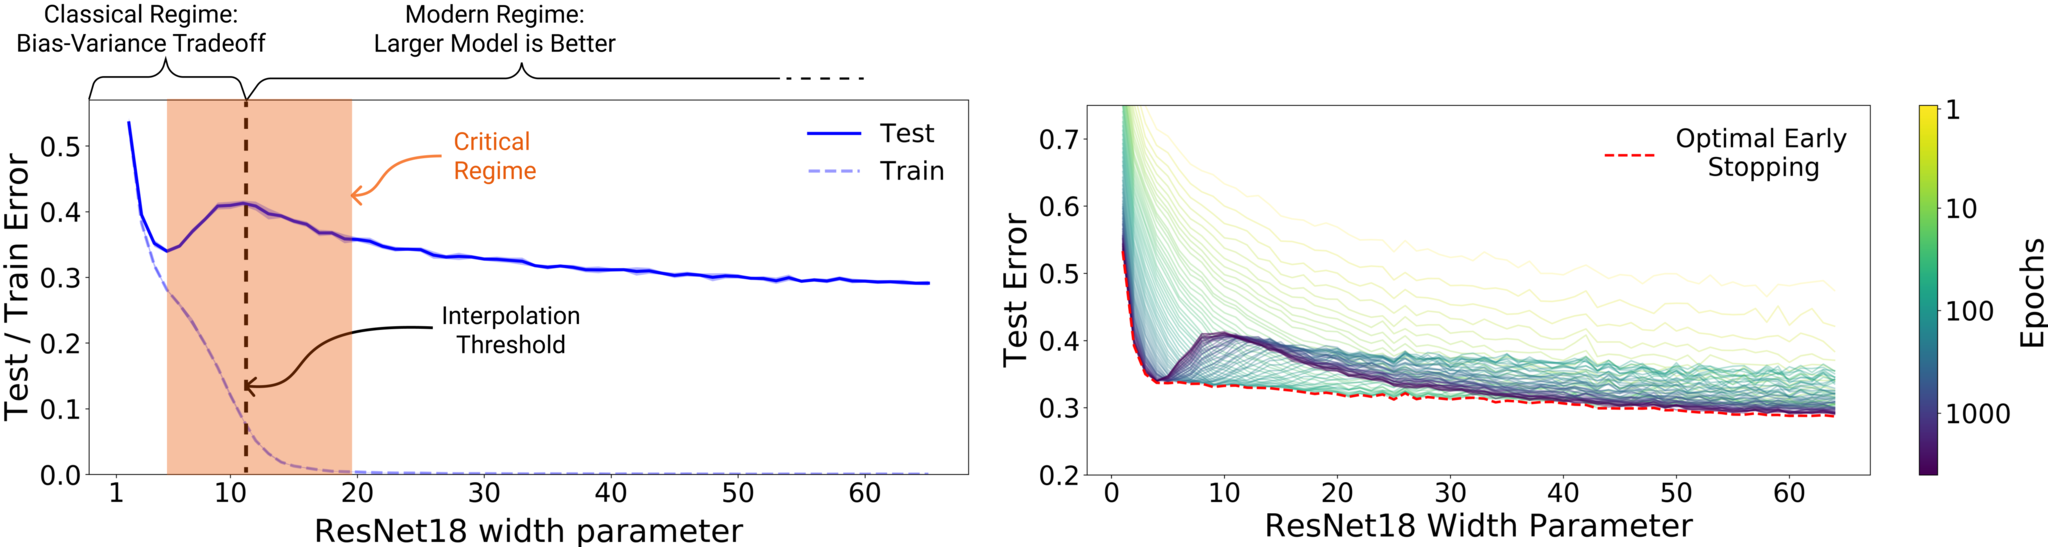
\includegraphics[width=0.98\linewidth,height=6.0cm,keepaspectratio]{assets/errorvscomplexity.png}\\[0.1ex]
{\scriptsize\color{uommuted}\textbf{Fig.~1, Nakkiran et al.\ (2019).} \textbf{Left:} test error on ResNet18s, varying width, CIFAR-10 + 15\% label noise. \textbf{Right:} test error coloured by training epoch; dashed red curve denotes optimal early stopping.}
\end{column}\hspace{0.01\linewidth}%
\begin{column}{0.36\linewidth}
\eyebrow{Thesis}
{\color{uomgrey}\textbf{\normalsize For modern training procedures the test-error curve exhibits \emph{two} descents,} separated by a sharp peak at the \kw{interpolation threshold} at which the procedure first fits the training set exactly.}\\[0.5ex]
\eyebrow{Beyond Section 5.3}
\small
The lecture introduces the phenomenon and links it to implicit regularisation. We extend this by substituting \emph{parameter count} with \kw{Effective Model Complexity} (EMC) -- the largest train-set size on which the procedure \(\T\) still drives training error below \(\varepsilon\) -- and demonstrating that the second descent occurs \kw{model-wise}, \kw{epoch-wise}, and \kw{sample-wise}, unified under the \kw{Generalised Double Descent Hypothesis}.\\[0.5ex]
\eyebrow{How to read Fig.\ 1}
\footnotesize
\begin{itemize}\setlength\itemsep{0.15ex}
\item[\textcolor{accentteal}{$\bullet$}] \kw{Classical regime} (left of peak): U-shape; classical bias-variance trade-off applies.
\item[\textcolor{accentcoral}{$\bullet$}] \kw{Critical regime} (coral band): test error \emph{spikes} near \(\mathrm{EMC}\!\approx\! n\); the \emph{interpolation threshold} sits at its centre.
\item[\textcolor{accentgreen}{$\bullet$}] \kw{Modern regime} (right of peak): test error \emph{descends a second time} as capacity grows.
\item[\textcolor{accentgold}{$\bullet$}] \kw{Dashed red curve} (right): optimal early stopping; tracks the descending epoch-wise envelope.
\end{itemize}
\end{column}
\end{columns}
\end{block}

\vspace{-0.2cm}

% =====================================================================
% ROW A (3 cols): Block 2 | Block 3 | Block 5
% =====================================================================
\begin{columns}[T,onlytextwidth]

% --- COL 1: Block 2 ---
\begin{column}{0.325\linewidth}
\begin{block}{\sectnum{2}Setting: the lecture decomposition we extend}
Following the course notation (Notes \S\,5.1, Eqs.~68--73):
\[\hat f \leftarrow \mathcal{A}(f;\Sset),\;
  R(f) := \E_{\bm{xy}}[\ell(\bm{y},f(\bm{x}))],\;
  \widehat R(f,\Sset) := \tfrac{1}{n}\sum_{i=1}^{n}\ell(\bm{y}_i,f(\bm{x}_i))\]
\(\hat f\) is found by gradient descent (Notes \S\,3.4):
\[\bm{\theta}_{t+1} \;=\; \bm{\theta}_t \;-\; \eta\,\nabla_{\bm{\theta}}\widehat R(f_{\bm{\theta}_t},\Sset)\]
The excess risk decomposes into three statistically meaningful gaps:
\[\underbrace{R(\hat f) - R(y^{*})}_{\text{excess risk}}
  = \underbrace{R(\hat f) - R(f_{\mathrm{erm}})}_{\text{\color{accentteal}\textbf{optimisation}}}
  + \underbrace{R(f_{\mathrm{erm}}) - R(f^{*})}_{\text{\color{accentgold}\textbf{estimation}}}
  + \underbrace{R(f^{*}) - R(y^{*})}_{\text{\color{accentblue}\textbf{approximation}}}\]
The classical bias-variance trade-off bundles \emph{approximation + part of estimation} into \kw{bias} and the rest into \kw{variance}; \emph{incomplete}, not wrong. The \kw{paper's pivot:} treat the entire procedure \(\T\) -- the data-to-classifier procedure parameterised by $\F$, optimiser, training time, regularisation, and label policy -- as the single object whose EMC matters.

\vspace{0.2ex}
\eyebrow{Term-by-term behaviour at the peak}
\footnotesize
\textcolor{accentteal}{\textbf{Approximation}} declines with training time as underfitting is dominated by \textbf{approximation error}; \textcolor{accentgold}{\textbf{estimation}} \emph{spikes} at \(\mathrm{EMC}\!\approx\! n\); \textcolor{accentblue}{\textbf{approximation}} declines with hypothesis-class size; All three terms co-exist and interact, i.e. a trade-off. 
\end{block}
\end{column}\hspace{0.005\linewidth}%

% --- COL 2: Block 3 ---
\begin{column}{0.325\linewidth}
\begin{block}{\sectnum{3}Definition + Hypothesis (Nakkiran et al.\ 2019)}
\eyebrow{Definition 1: Effective Model Complexity}
A \kw{training procedure} \(\T\) maps any labelled train set \(S = \{(\bm{x}_i,\bm{y}_i)\}_{i=1}^{n}\) to a classifier \(\T(S)\). For an error tolerance \(\varepsilon>0\),
\[\boxed{\;\mathrm{EMC}_{\D,\varepsilon}(\T)\;:=\;\max\bigl\{\,n\;\bigm|\;\E_{S\sim\D^{n}}\bigl[\mathrm{Error}_{S}(\T(S))\bigr]\le\varepsilon\,\bigr\}\;}\]
i.e.\ the largest sample size on which \(\T\) drives train error below \(\varepsilon\). Note that \(\mathrm{EMC}\) depends on the optimiser, training time, augmentation, and labels.

\vspace{0.3ex}
\eyebrow{Hypothesis 1: Generalised Double Descent}
For ``natural'' \(\D\), neural-network procedures \(\T\), and small \(\varepsilon\) (paper: \(\varepsilon=0.1\)):
\begin{itemize}\setlength\itemsep{0.2ex}
\item[\chip{accentteal}{$\mathrm{EMC}\!\ll\! n$}] \kw{Under-parameterised:} any change to \(\T\) that \emph{increases} EMC \emph{decreases} test error.
\item[\chip{accentcoral}{$\mathrm{EMC}\!\approx\! n$}] \kw{Critically parameterised:} the sign of the same change is \emph{indeterminate}.
\item[\chip{accentgreen}{$\mathrm{EMC}\!\gg\! n$}] \kw{Over-parameterised:} any change to \(\T\) that \emph{increases} EMC \emph{decreases} test error.
\end{itemize}

\HypBox{\textbf{Why this is a hypothesis, not a theorem.} \(\varepsilon\) and ``sufficiently smaller / larger'' are heuristic; the critical-interval width is not formally specified for deep nets. \kw{EMC is operational, not predictive}: peak location must be \emph{measured}, not derived.}
\end{block}
\end{column}\hspace{0.005\linewidth}%

% --- COL 3: Block 5 (Sample-wise) ---
\begin{column}{0.325\linewidth}
\begin{block}{\sectnum{5}Sample-wise descent: increasing \(n\) can locally raise test loss}
\centering
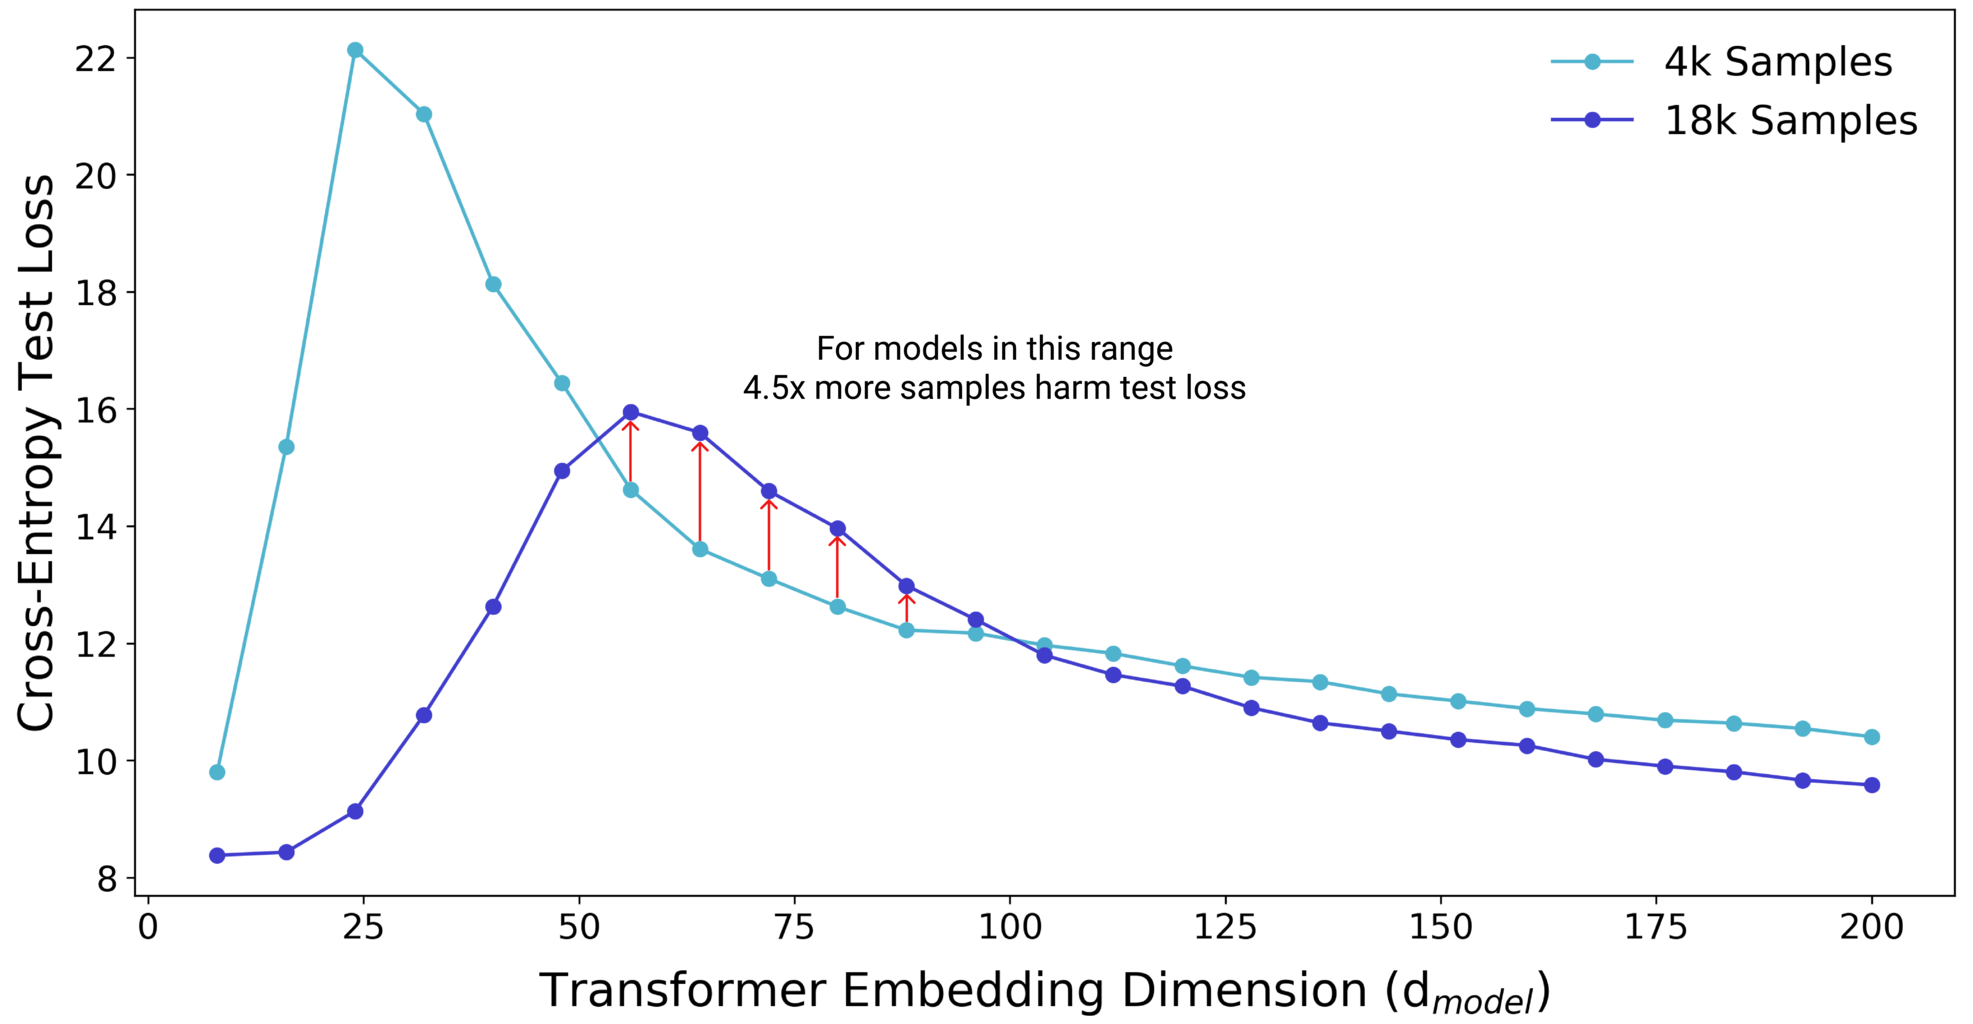
\includegraphics[width=0.96\linewidth,height=4.8cm,keepaspectratio]{assets/NLP-small-data-vary-MDD.png}\\[0.1ex]
{\scriptsize\color{uommuted}\textbf{Fig.~3, Nakkiran et al.} IWSLT'14 De-En, 6-layer Transformer, \(d_{\text{ff}}\!=\!4d_{\text{model}}\), 80k gradient steps, 10\% label smoothing. Highlighted bars indicate the \(d_{\text{model}}\) interval over which a 4.5\(\times\) increase in \(n\) \emph{raises} test loss.}
\justifying
\vspace{0.2ex}
\begin{itemize}\setlength\itemsep{0.2ex}
\item Fixing \((\T,f)\) and increasing \(n\) increases EMC; widths near the interpolation threshold are thereby displaced into the critical regime.
\item The non-monotonicity is local: asymptotically, additional samples reduce empirical risk.
\item \kw{Practical implication:} an \kw{ensemble of models trained on disjoint sub-samples} sits past each member's peak; averaging cancels member-specific interpolation noise (Fig.~28).
\end{itemize}
\end{block}
\end{column}

\end{columns}

\vspace{-0.3cm}

% =====================================================================
% WIDE ROW: Block 4 (Heatmaps - full width with internal 3 columns)
% =====================================================================
\begin{block}{\sectnum{4}Main empirical evidence: model-wise \(\times\) epoch-wise double descent}
\begin{columns}[T,onlytextwidth]
\begin{column}{0.30\linewidth}
\centering
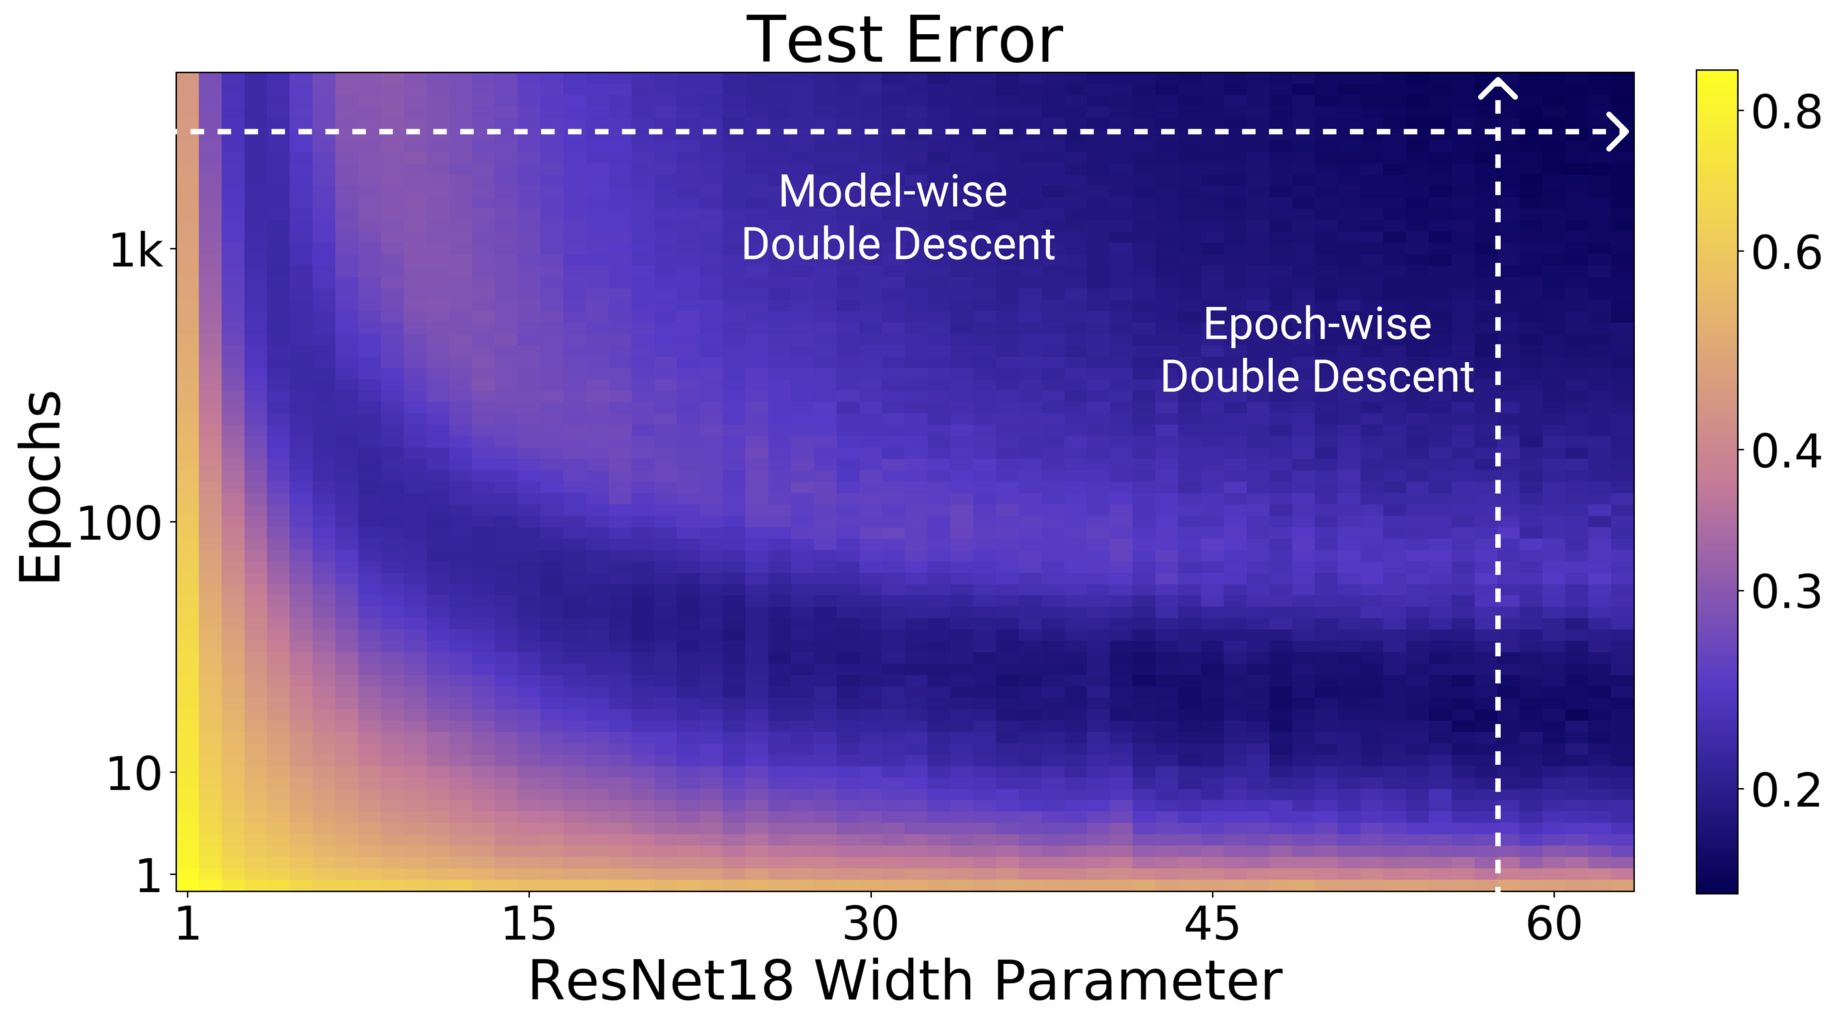
\includegraphics[width=0.98\linewidth,height=5.4cm,keepaspectratio]{assets/Intro-ocean-test.png}\\[0.1ex]
{\scriptsize\color{uommuted}\textbf{Fig.~2 (left), test error.} Test error attains \(\approx\) 0.47 at width \(k\!\approx\!10\) and decreases to \(\approx\) 0.24 at \(k\!=\!64\).}
\end{column}\hspace{0.01\linewidth}%
\begin{column}{0.30\linewidth}
\centering
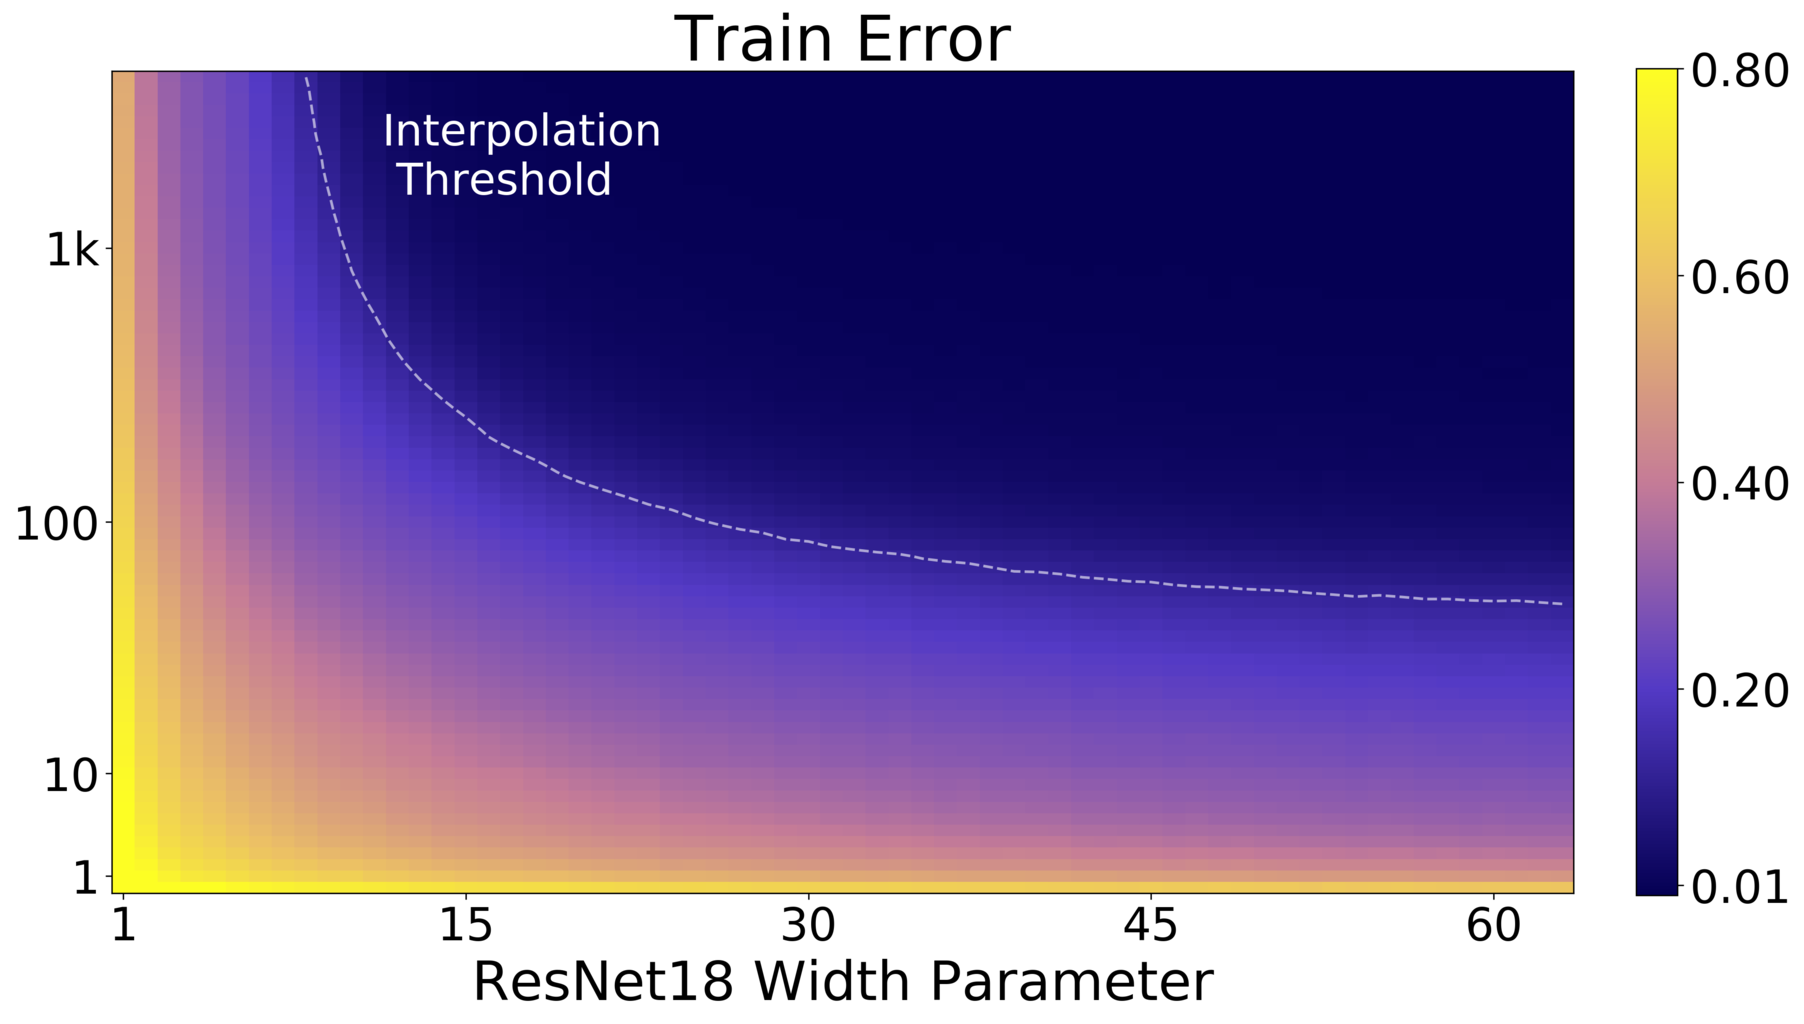
\includegraphics[width=0.98\linewidth,height=5.4cm,keepaspectratio]{assets/Rn-cifar10-p15-adam-aug-train.png}\\[0.1ex]
{\scriptsize\color{uommuted}\textbf{Fig.~2 (right), train error.} Dashed curve denotes the interpolation threshold (\(\widehat R\!\to\!0\)).}
\end{column}\hspace{0.01\linewidth}%
\begin{column}{0.37\linewidth}
\eyebrow{Reading the heatmaps}
\footnotesize
\begin{itemize}\setlength\itemsep{0.15ex}
\item \kw{Same axes:} ResNet18 width \(k\!\in\![1,64]\) vs training epochs (log).
\item \kw{Horizontal slice:} \chip{accentcoral}{model-wise} peak as width grows. \kw{Vertical slice:} \chip{accentteal}{epoch-wise} peak as training continues.
\item \kw{Key alignment:} the locus of high test error in the left heatmap coincides with the train-interpolation contour (dashed) in the right heatmap; the peak occurs \emph{at} the threshold, not past it.
\end{itemize}
\eyebrow{Setup + key numbers (paper \S\,4)}
\footnotesize
ResNet18, CIFAR-10, \kw{15\% label noise}, augmentation, Adam (lr 1e-4), 4k epochs. Sample-wise (Fig.~3): a \kw{4.5\(\times\) data increase} (4k\(\to\)18k) raises test loss for \(d_{\text{model}}\!\in\![0,200]\). Paper uses \kw{\(\varepsilon\!=\!0.1\)}.

\vspace{0.3ex}
\takeaway{The unifying variable is EMC: any modification of \(\T\) that moves EMC across \(n\) shifts the peak correspondingly.}
\end{column}
\end{columns}
\end{block}

\vspace{-0.35cm}

% =====================================================================
% ROW B (3 cols): Block 6 | Block 7 | Block 8
% =====================================================================
\begin{columns}[T,onlytextwidth]

% --- COL 1: Block 6 (Mechanism) ---
\begin{column}{0.325\linewidth}
\begin{block}{\sectnum{6}Mechanism (rigorous for linear models; conjectural for deep nets)}
\eyebrow{Critically parameterised} The hypothesis class admits effectively a unique interpolant. Constraining it to fit noisy or mis-specified labels perturbs the on-distribution map; test risk consequently spikes.

\vspace{0.2ex}
\eyebrow{Over-parameterised} A continuum of interpolants exists. The optimiser's \kw{implicit bias} (e.g.\ SGD toward minimum-norm) selects an interpolant that absorbs label noise while preserving smoothness on the data manifold.

\vspace{0.4ex}
\centering
\begin{tikzpicture}[every node/.style={font=\scriptsize},x=0.31\linewidth,y=0.55cm]
  % Three regime bands with rounded corners
  \fill[accentteal!18,rounded corners=2pt] (0,0) rectangle (0.95,0.55);
  \fill[accentcoral!50,rounded corners=2pt] (1.0,0) rectangle (1.5,0.55);
  \fill[accentgreen!22,rounded corners=2pt] (1.55,0) rectangle (2.5,0.55);
  % Top labels (regime expressions)
  \node[anchor=south,color=accentteal] at (0.475,0.6) {\bfseries\scriptsize $\mathrm{EMC}\!\ll\! n$};
  \node[anchor=south,color=accentcoral] at (1.25,0.6) {\bfseries\scriptsize $\mathrm{EMC}\!\approx\! n$};
  \node[anchor=south,color=accentgreen] at (2.025,0.6) {\bfseries\scriptsize $\mathrm{EMC}\!\gg\! n$};
  % Inside-band labels
  \node[anchor=center] at (0.475,0.275) {\bfseries\scriptsize unique interpolant};
  \node[anchor=center,color=white] at (1.25,0.275) {\bfseries\scriptsize peak};
  \node[anchor=center] at (2.025,0.275) {\bfseries\scriptsize continuum};
  % Bottom labels (intuition)
  \node[anchor=north] at (0.475,-0.05) {\scriptsize classical U-curve};
  \node[anchor=north,color=accentcoral] at (1.25,-0.05) {\scriptsize\itshape critical regime};
  \node[anchor=north] at (2.025,-0.05) {\scriptsize implicit bias selects};
\end{tikzpicture}

\justifying
\vspace{0.3ex}
\eyebrow{Where the mechanism is proven}
Mei \& Montanari (2022, Thm.~2) establish a test-risk peak at \(d{=}n\) for random-features regression under mis-specification; Belkin et al.\ (2019) prove an analogous peak for least-squares; Bartlett et al.\ (2020) prove benign overfitting under minimum-norm interpolation. The deep-network analogue remains conjectural.
\end{block}
\end{column}\hspace{0.005\linewidth}%

% --- COL 2: Block 7 (Critical reflection) ---
\begin{column}{0.325\linewidth}
\begin{block}{\sectnum{7}Critical reflection: what we do \emph{not} claim}
\begin{itemize}\setlength\itemsep{0.4ex}
\item \kw{The bias-variance trade-off is not invalidated.} It remains correct within a fixed hypothesis class; it is \emph{incomplete} once \(\T\) is permitted to vary.
\item \kw{Model width, training time, and sample size are not monotonic in test risk.} Within the critical interval each can locally \emph{increase} it.
\item \kw{Label noise is not the cause of the peak.} Noise amplifies it; the peak persists at \kw{0\% noise} (CIFAR-100, Fig.~4a; CNN, Fig.~7) under model mis-specification.
\item \kw{Parameter count does not equal EMC.} Parameters constitute one input to EMC; optimiser, epochs, augmentation, and label policy contribute jointly.
\end{itemize}
\end{block}
\end{column}\hspace{0.005\linewidth}%

% --- COL 3: Block 8 (Practical + Open) ---
\begin{column}{0.325\linewidth}
\begin{block}{\sectnum{8}Practical implications and open questions}
\eyebrow{Implications for practice}
\begin{itemize}\setlength\itemsep{0.2ex}
\item \kw{Diagnostic.} Train and test curves decouple near the interpolation threshold; monitor both.
\item \kw{Per-model mitigation.} Weight decay, early stopping, or scaling well beyond the threshold.
\item \kw{Aggregate mitigation.} Ensemble \(K\) sub-sampled models, each over-parameterised relative to its own \(n\) (Fig.~28).
\item \kw{Augmentation.} Data augmentation shifts the peak rightward (Fig.~5) without changing the architecture.
\end{itemize}
\eyebrow{Open scientific questions}
\begin{itemize}\setlength\itemsep{0.2ex}
\item A principled choice of \(\varepsilon\) and closed-form critical-interval width.
\item A non-linear EMC theorem for over-parameterised networks.
\item Characterisation of SGD's implicit bias for realistic architectures and losses.
\end{itemize}
\end{block}
\end{column}

\end{columns}

\vspace{0.05cm}
\bigtakeaway{Interpolation is a threshold to understand, not a final verdict.}
\vspace{0.1cm}

% =====================================================================
% FOOTER: References + AI declaration (full width, two columns)
% =====================================================================
\begin{columns}[T,onlytextwidth]
\begin{column}{0.72\linewidth}
\eyebrow{Key references} \scriptsize
[1]~Nakkiran et al. \emph{Deep Double Descent.} 2019.
[2]~Belkin et al. \emph{Reconciling ML practice \& bias-variance.} 2019.
[3]~Zhang et al. \emph{Rethinking generalization.} 2017.
[4]~Mei \& Montanari. 2022.
[5]~Bartlett et al. 2020.
[6]~Brown \& Mukherjee. 2026.
\end{column}
\begin{column}{0.26\linewidth}
\eyebrow{AI-use} \scriptsize
AI used for \LaTeX{} typesetting only. All content and refs verified by authors. Figs 1--3 from [1].
\end{column}
\end{columns}

\end{frame}
\end{document}
